%% entwurf.tex
%% $Id: entwurf.tex 61 2012-05-03 13:58:03Z bless $
%%

\chapter{Conceptual Design and Implementation}
\label{ch:Conceptual Design}
%% ==============================
\par{
Without further ado, design and implementation of the initial ideas began. As Section \ref{ch:Analysis} showed, there are some potentially promising improvements to be made to run length encoding, but how well they scale and work on a larger input with versatile symbols or bytes has to be determined.
}
%% ==============================
\section{Preprocessing}
%% ==============================
\label{ch:Conceptual Design:sec:Preprocessing}

%% ==============================
\subsection{Vertical Byte Reading}
%% ==============================
\label{ch:Conceptual Design:sec:Parallel Byte Reading}
\par{
Implementing the vertical reading of the input shown in Section \ref{ch:Analysis:sec:Improvements by Preprocessing:subSec:vertReading} was not hard but it should be kept in mind that the size of the input chunks has to be divisible by the size of 8. Otherwise parsing it into an Array of Bytes results in the last Byte having some padding which might cause problems later on.  By collecting the bits into a proprietary data structure, we avoid this problem but working with bytes internally should be easier. For larger files it should also be possible to work in space and writing the output on the fly during the reading process. Nonetheless both ways of collecting all bits of identical significance and writing on the fly are implemented.}

\subsubsection{First Ideas}
\par{
Initially some other ideas have been followed with very poor results. One idea was arranging all input bits in a Matrix or square Matrix in a way it would still be receivable later on. This way other methods from linear algebra would have been applicable to the input data, so that the construction of a triangular matrix or other preprocessing would result in long runs of zeros. Difficulties in the construction and transformation of the Data lead to the abandonment of this approach and the already described vertical interpretation was used further on.}

\subsubsection{Other Difficulties}
\par{
Other difficulties arose while performing bit operations, because it became slow on larger workloads. \\

TODO: explain used \href{https://discuss.kotlinlang.org/t/i-o-streams-for-kotlin/9802}{lib}}

\subsubsection{Compression improvements trough vertical reading}
\par{
First results of just plain binary RLE on the vertical interpretation improved its overall performance and achieved a small edge over regular binary RLE with a slightly smaller expansion but it is still not as good as byte wise RLE with a small run value of 2 bits.
\begin{table}[H]
	\centering
	\begin{tabular}{r|r|r}	
		bits per rle number & ratio in \% & bits per symbol in $\frac{bits}{symbol}$\\
		\hline
		8 & 255.22 & 20.41\\
		7 & 224.45 & 17.95\\
		6 & 194.74 & 15.57\\
		5 & 167.04 & 13.36\\
		4 & 142.58 & 11.40\\
		3 & 127.80 & 10.22\\
		2 & 139.79 & 11.18 \\
	\end{tabular}
	\caption{Binary RLE on vertical interpreted data}
	\label{tab:t30 binary RLE on vertical interpreted data}
\end{table}
}

\par{
If we take a closer look on each file, we see similar results compared to the original proposed binary RLE, where most files had a compression ratio of just above 1 with 3 bits per RLE encoded number, except for the file \textit{pic}. Average sizes are increasing again with more bits per run up to 2.5 times its original size and also the file \textit{pic} has the best compression ratio. This time although it is at its peak using 6 bits per RLE run and only achieves a compression of 3.67 $\frac{bits}{symbol}$ compared to 1.56 $\frac{bits}{symbol}$ with simple binary RLE. These results were already better than the simple binary RLE but they were still quite far from the desired outcome. This mainly arose because increasing the bits per run improved the result for the most significant bits but also degraded the results for the other bits. So the idea of encoding the bits of different significance with different RLE schemes with varying bits per run to solve this issue.  
}

\subsection{Varying maximum run lengths}
\label{ch:Conceptual Design:sec:var lengths}
\par{
This time the most significant bits have been encoded with more bits per run than the other ones and after bench marking every combination, it turned out, with 2 bits per run and 5 bits per run for the 3 most significant bits, it improved by another 4 percent. Now most files have a $\frac{bits}{symbol}$ ratio of only slightly above 9. More specifically some textual files are close to 8, which relates to the earlier mentioned ASCII fragments in UTF-8 encoding. This time higher possible runs on this position resulted in fewer runs in total, so in a better compression overall. Applying this increase to more than the most significant bit lead to a decrease in performance, which most likely related to the shorter runs on lower order bits, seen in Section \ref{ch:Analysis:sec:Improvements by Preprocessing:subSec:vertReading}. Therefore this idea was applied again but with a much finer granularity and every combination of different run lengths of every bit could be tried out. Also the concept of mapping the input to lower value bytes to artificially increase runs of consecutive zeros on more significant bits should be applied first.
}
\par{
Testing out every combination of different run lengths would imply running $8^6$ combinations because every of the 8 bits could be encoded with 2 to 7 bits per run, totaling at $2097152$ possible combinations. Assuming around 10 seconds for each encoding round would still result in somewhat around $6000h$ of computing which is clearly to much. Even using multi-threading would not completely resolve this issue so the computation had to be further reduced. By trying only a few specific combinations we assume to be good, we can then selectively small changes to improve further.
This way the results were improved to $XXX$ but this was still far from the desired state. Most files still increased in size even though all bits could be encoded differently. To increase runs overall, the already described byte mapping was applied to the input data.
}

\subsection{Byte remapping}
\par{
As shown in Section \ref{ch:Analysis:sec:Improvements by Preprocessing:subSec:byteRemapping} this effect could become useful if it resulted in longer runs. This effect was also seen in the second and third most significant bit, as higher value bytes became unlikely in the input data after the remapping so the idea of varying maximum run lengths for different significant bits became more appealing again. To determine the best combination of maximum run lengths and how many most significant bits should be encoded with a higher maximum run length, all combinations of these were tested and the results plotted below.
}
\begin{figure}[H]
%\begin{scaletikzpicturetowidth}{\textwidth}
%\resizebox{\textwidth}{!}{
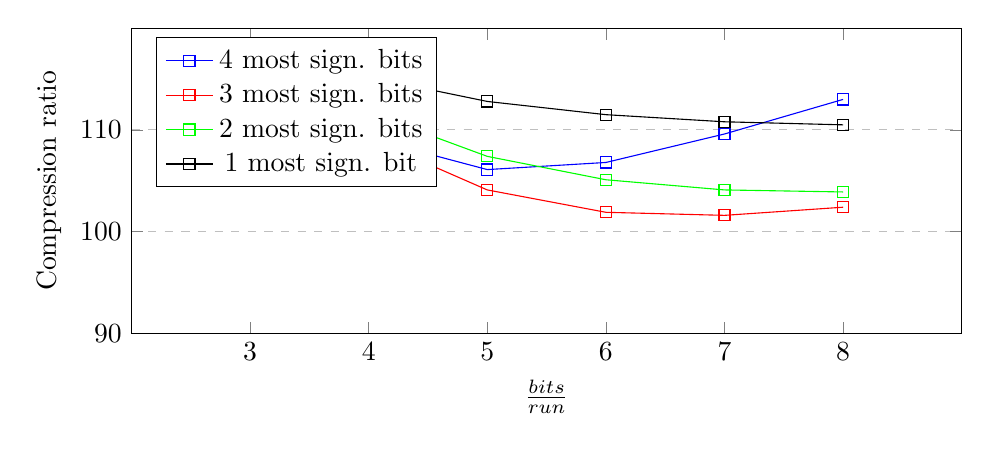
\begin{tikzpicture}%[scale=\tikzscale]
\begin{axis}[
width=\textwidth,
height=0.45\textwidth,
xlabel={$\frac{bits}{run}$},
ylabel={Compression ratio},
xmin=2, xmax=9,
ymin=90, ymax=120,
xtick={3,4,5,6,7,8},
ytick={90,100,110},
legend pos=north west,
ymajorgrids=true,
grid style=dashed,
]
\addplot[
	color=blue,
	mark=square,
	]
	coordinates {
		(4,109.2)(5,106.1)(6,106.8)(7,109.6)(8,113)
	};
\addplot[
	color=red,
	mark=square,
	]
	coordinates {
		(4,109.2)(5,104.1)(6,101.9)(7,101.6)(8,102.4)
	};
\addplot[
	color=green,
	mark=square,
	]
	coordinates {
		(4,111.7)(5,107.4)(6,105.1)(7,104.1)(8,103.9)
	};
\addplot[
	color=black,
	mark=square,
	]
	coordinates {
		(4,115.2)(5,112.8)(6,111.5)(7,110.8)(8,110.5)
	};
	\legend{4 most sign. bits,3 most sign. bits,2 most sign. bits, 1 most sign. bit}
\end{axis}
\end{tikzpicture}
%}
%\end{scaletikzpicturetowidth}
\caption{Different run lengths for byte mapping and varying maximum run lengths}
\label{fig:2:different run lengths for byte mapping and varying maximum run lengths}
\end{figure}

\par{
The combination of 3 bits per run and 7 bits per run for the 3 most significant bits yielded the overall best results with 101.6\% of its original size and 8.13 $\frac{bits}{symbol}$ as shown in Figure \ref{fig:2:different run lengths for byte mapping and varying maximum run lengths}. It has to be mentioned, that the expected overhead is rather small but the increase in average run length lead to a reduction in size which was still not really compressing. Some files got a little smaller while other files almost doubled in size which is still no real enhancement over regular rle which performs really well on specific files.
\begin{table}[H]
	\centering
	\begin{tabular}{r|r|r|r|r}	
		file & size original & size encoded & ratio in \% & $\frac{bits}{symbol}$\\
		\hline
		bib & 111261 & 97867 & 87.96 & 7.03\\
		book1 & 768771 & 579649 & 75.39 & 6.03 \\
		book2 & 610856 & 484989 & 79.39 & 6.35\\
		geo & 102400 & 116487 & 113.75 & 9.10\\
		news & 377109 & 315446 & 83.64 & 6.69\\
		obj1 & 21504 & 23871 & 111.00 & 8.88\\
		obj2& 246814 & 276301 & 111.94 & 8.95\\		 
		paper1 & 53161 & 43556 & 81.93 & 6.55\\		 
		paper2& 82199 & 62544 & 76.08 & 6.08\\		 
		pic & 513216 & 272034 & 53.00 & 4.24\\		 
		progc & 39611 & 33073 & 83.49 & 6.67\\		 
		progl & 71646 & 53653 & 74.88 & 5.99\\		 
		progp & 49379 & 39400 & 79.79 & 6.38\\		 
		trans & 93695 & 84494 & 90.17 & 7.21\\
		\hline
		all files & 3145718 & 2487460 & 79.07 & 6.32
	\end{tabular}
	\caption{Calgary Corpus encoded with vertical reading, byte remapping and 2 bits per RLE run and 5 for the 3 most significance bits}
\label{tab:t43 Calgary Corpus encoded with vertical reading, byte remapping and 2 bits per RLE run and 5 for the 3 most significance bits}
\end{table}

2020-01-13 21:39:50 INFO/Analyzer  Corpus size original: 3145718 // 3.145718 Mb  
2020-01-13 21:39:50 INFO/Analyzer  Corpus size encoded: 3197179 // 3.197179 Mb  
2020-01-13 21:39:50 INFO/Analyzer  1.0163590633362558 compression ratio  
2020-01-13 21:39:50 INFO/Analyzer  with 8.130872506690046 bits/symbol  
2020-01-13 21:39:50 INFO/Analyzer  File bib, size original: 111261, size encoded: 127820, compression: 114.8830228022398, bps: 9.190641824179183  
2020-01-13 21:39:50 INFO/Analyzer  File book1, size original: 768771, size encoded: 735120, compression: 95.62275371989838, bps: 7.64982029759187  
2020-01-13 21:39:50 INFO/Analyzer  File book2, size original: 610856, size encoded: 623881, compression: 102.13225375538588, bps: 8.17058030043087  
2020-01-13 21:39:50 INFO/Analyzer  File geo, size original: 102400, size encoded: 159874, compression: 156.126953125, bps: 12.49015625  
2020-01-13 21:39:50 INFO/Analyzer  File news, size original: 377109, size encoded: 407185, compression: 107.97541294426811, bps: 8.638033035541449  
2020-01-13 21:39:50 INFO/Analyzer  File obj1, size original: 21504, size encoded: 31871, compression: 148.20963541666669, bps: 11.856770833333334  
2020-01-13 21:39:50 INFO/Analyzer  File obj2, size original: 246814, size encoded: 369726, compression: 149.7994441158119, bps: 11.983955529264952  
2020-01-13 21:39:50 INFO/Analyzer  File paper1, size original: 53161, size encoded: 56323, compression: 105.94796937604636, bps: 8.475837550083709  
2020-01-13 21:39:50 INFO/Analyzer  File paper2, size original: 82199, size encoded: 79621, compression: 96.86370880424336, bps: 7.749096704339469  
2020-01-13 21:39:50 INFO/Analyzer  File pic, size original: 513216, size encoded: 330347, compression: 64.36802437959845, bps: 5.149441950367876  
2020-01-13 21:39:50 INFO/Analyzer  File progc, size original: 39611, size encoded: 42454, compression: 107.17729923506096, bps: 8.574183938804877  
2020-01-13 21:39:50 INFO/Analyzer  File progl, size original: 71646, size encoded: 68051, compression: 94.98227395807163, bps: 7.59858191664573  
2020-01-13 21:39:50 INFO/Analyzer  File progp, size original: 49379, size encoded: 50333, compression: 101.93199538265254, bps: 8.154559630612203  
2020-01-13 21:39:50 INFO/Analyzer  File trans, size original: 93695, size encoded: 110477, compression: 117.91130796734083, bps: 9.432904637387267 
}

\subsection{Burrows-Wheeler-Transformation Appliance}
\par{
Another possible preprocessing step which promised an improvement is the mentioned Burrows-Wheeler-Transformation from Section \ref{ch:Principles of compression:sec:Other:subSec:bwt}, initially applied to regular binary and byte wise RLE. By mistake a very simple transformation implementation was chosen, working by adding additional start and stop symbols to the input string (0x02 as STX, start of text and 0x03 as ETX, end of text). Some basic testing and playing around worked great but later on it revealed some major issues. For example the Calgary Corpus consists of more than textual data, in fact the files geo, obj1, obj2 and pic contain of some binary data of include the symbols STX or ETX so we wont be able to apply the transformation to these. Another shortcoming was the very poor time complexity of almost $O (n^2)$ because under the hood, it uses a dual pivot Quick-sort algorithm from the JDK 11, which is typically faster than traditional one pivot Quick-sort. This algorithm offers $\Theta (n \: log(n))$ average time complexity but in the worst case, its time complexity is cubic. This problem was partially solved by reading the input data in parts and performing the transformation on each part, result in a much smaller length $n$ and thus better run time at the expense of a slightly worse transformation result. As all chunks are individual transformations, they can also be computed in parallel without much effort.

\begin{table}[H]
	\centering
	\begin{tabular}{r|r|r}	
		bits per rle number & ratio in \% & bits per symbol in $\frac{bits}{symbol}$\\
		\hline
		3 & 95.41 & 7.63\\
		2 & 91.39 & 7.31 \\
	\end{tabular}
	\caption{Initial BWT implementation on byte wise RLE}
	\label{tab:t11 Simple Burrows Wheeler Transformation on byte wise RLE}
\end{table}
}
\par{
While it was only applicable to textual data and very slow, even when divided into smaller parts and computed in parallel, it improved the overall results of byte wise RLE by 16\% to a compression ratio of slightly over 7 $\frac{bits}{symbol}$ which seemed like a good start. Regular binary RLE did not really benefit from this transformation as expected but on vertical interpretation, consecutive characters result in successive bits on every significance. Still this implementation had to be dropped and switched against one that could handle arbitrary input to be able to transform all files. This time all files could be processed and the resulting compression with byte wise RLE improved further.

\begin{table}[H]
	\centering
	\begin{tabular}{r|r|r}	
		bits per rle number & ratio in \% & bits per symbol in $\frac{bits}{symbol}$\\
		\hline
		3 & 91.62 & 7.33\\
		2 & 89.46 & 7.15
	\end{tabular}
	\caption{Burrows Wheeler Transformation on byte wise RLE}
	\label{tab:t12 Burrows Wheeler Transformation on byte wise RLE}
\end{table}
}

\par{
In Section \ref{ch:Principles of compression:sec:Other} the Burrows-Wheeler-Transformation inversion was performed using a Matrix M containing all cyclic rotations of the input word, sorted in lexicographic order. However this is has a bad complexity and the inverting process does not even has access to this Matrix M.\\

TODO: explain creation using suffix array \\
}

\par{
In general a Burrows-Wheeler-Transformation should also increase the runs in the implementation of Section \ref{ch:Analysis:sec:Improvements by Preprocessing:subSec:vertReading} and \ref{ch:Analysis:sec:Improvements by Preprocessing:subSec:byteRemapping} so those preprocessing steps were also applied in combination. To do so, it was first swapped against an sufficient implementation provided by a paper from m. Burrows and D. J. Wheeler \cite{Burrows94} from 1994. Their method is also the one described in Section \ref{ch:Analysis:sec:Improvements by Preprocessing:subSec:bwt} and could handle arbitrary input but it also had some downsides like the additional index $I$ of the transformation, which had to be persisted as well. The major downside of this implementation although was the rather slow. To overcome this issue and the saving of additional indices, the implementation used had to be swapped once more against one that was first described by \cite{Burrows-linear-time} in 2009.

TODO: explain inversion using Lyndon words
}
\par{
Swapping the implementation resulted in way better results, even with the simple regular RLE archiving compression ratios around 60 \% of its original size was possible while using 4 bits per run. This was mainly because of the longer repetitions possible after the transformation was performed on the whole input instead of small chunks. Another reason is the lack of additional information needed to store because we do no longer need to store the transformation index of every chunk.
	\begin{table}[H]
		\centering
		\begin{tabular}{r|r|r}	
			bits per rle number & ratio in \% & bits per symbol in $\frac{bits}{symbol}$\\
			\hline
			8 & 74.5 & 5.96\\
			7 & 70.0 & 5.60\\
			6 & 65.7 & 5.25\\
			5 & 61.8 & 4.98\\
			4 & 59.9 & 4.81\\
			3 & 61.3 & 4.94\\
			2 & 69.8 & 5.42
		\end{tabular}
		\caption{Modified Burrows Wheeler Transformation on byte wise RLE}
		\label{tab:t12 Modified Burrows Wheeler Transformation on byte wise RLE}
	\end{table}
}


\par{
Using the modified bijective Burrows-Wheeler-Transformation, regular binary and byte-wise RLE had their peak performance while using 4 bits per encoded number but interestingly the vertical encoded RLE did not. Instead it maxed out with 4 bits per encoded number with 67 \% of its original size with only 5.42 $\frac{bits}{symbol}$. Combining the byte mapping and the transformation yielded slightly better results with 65 \% and 5.22 $\frac{bits}{symbol}$ as show in Figure \ref{fig:3:Different run lengths with and without transformations}. There was still room for some optimizations because as seen in Section \ref{ch:Conceptual Design:sec:var lengths}, the remapping of the input resulted in longer runs on the higher order bits and the vertical interpretation made it possible to encode different sections with different maximum run lengths.

TODO: make both plots align side by side
\begin{figure}[H]
	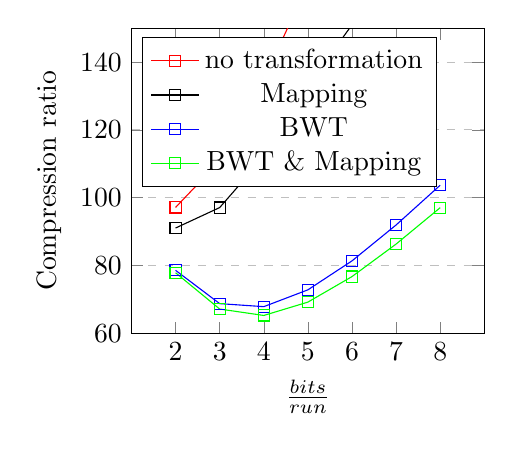
\begin{tikzpicture}[scale=1]
	\begin{axis}[
	width=.5\textwidth,
	height=0.45\textwidth,
	xlabel={$\frac{bits}{run}$},
	ylabel={Compression ratio},
	xmin=1, xmax=9,
	ymin=60, ymax=150,
	xtick={2,3,4,5,6,7,8},
	ytick={60,80,100,120,140},
	legend pos=north west,
	ymajorgrids=true,
	grid style=dashed,
	]
	\addplot[
	color=red,
	mark=square,
	]
	coordinates {
		(2,97.14)(3,110.82)(4,134.83)(5,163)(6,192)
	};
	\addplot[
	color=black,
	mark=square,
	]
	coordinates {
		(2,91.06)(3,97.1)(4,112)(5,133)(6,151)
	};
	\addplot[
	color=blue,
	mark=square,
	]
	coordinates {
		(2,78.58)(3,68.76)(4,67.87)(5,72.83)(6,81.37)(7,91.96)(8,103.69)
	};
	\addplot[
	color=green,
	mark=square,
	]
	coordinates {
		(2,77.87)(3,67.17)(4,65.27)(5,69.21)(6,76.74)(7,86.33)(8,97.07)
	};
	\legend{no transformation,Mapping,BWT,BWT \& Mapping}
	\end{axis}
	\end{tikzpicture}
	\caption{Different run lengths with and without transformations}
	\label{fig:3:Different run lengths with and without transformations}
	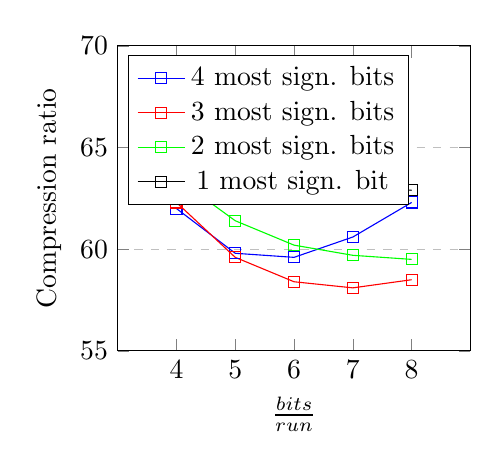
\begin{tikzpicture}[scale=1]
	\begin{axis}[
	width=.5\textwidth,
	height=0.45\textwidth,
	xlabel={$\frac{bits}{run}$},
	ylabel={Compression ratio},
	xmin=3, xmax=9,
	ymin=55, ymax=70,
	xtick={4,5,6,7,8},
	ytick={55,60,65,70},
	legend pos=north west,
	ymajorgrids=true,
	grid style=dashed,
	]
	\addplot[
	color=blue,
	mark=square,
	]
	coordinates {
		(4,62)(5,59.8)(6,59.6)(7,60.6)(8,62.3)
	};
	\addplot[
	color=red,
	mark=square,
	]
	coordinates {
		(4,62.3)(5,59.6)(6,58.4)(7,58.1)(8,58.5)
	};
	\addplot[
	color=green,
	mark=square,
	]
	coordinates {
		(4,63.5)(5,61.4)(6,60.2)(7,59.7)(8,59.5)
	};
	\addplot[
	color=black,
	mark=square,
	]
	coordinates {
		(4,65.2)(5,64.1)(6,63.4)(7,63.0)(8,62.9)
	};
	\legend{4 most sign. bits,3 most sign. bits,2 most sign. bits, 1 most sign. bit}
	\end{axis}
	\end{tikzpicture}
	\caption{Different run lengths for byte mapping and transformation and varying maximum run lengths}
	\label{fig:4:Different run lengths for byte mapping and transformation and varying maximum run lengths}
\end{figure}
}

\par{
In Section \ref{ch:Conceptual Design:sec:var lengths} different run lengths for different significant bits provided an edge over just fixed maximum run length, so this combination was also tried out. After testing all combinations of possible and reasonable variables it was found that using a Burrows-Wheeler-Transformation and byte remapping as preprocessing steps, parse the transformed data in vertical order and then using 3 bits per run for low significant bits and 7 for the 3 most significant bits, run length encoding performs at its peak. Using this setup, the Calgary Corpus can be compressed down to 58.1 \% of its original size while using only 4.65 $\frac{bits}{symbol}$ as shown in figure \ref{fig:4:Different run lengths for byte mapping and transformation and varying maximum run lengths}. This was the best result achieved so far and the detailed compression results are shown below.

TODO: reevaluate results after bug!!!
\begin{table}[H]
	\centering
	\begin{tabular}{r|r|r|r|r}	
		file & size original & size encoded & ratio in \% & $\frac{bits}{symbol}$\\
		\hline
		bib & 111261 & 62791 & 56.43 & 4.51\\
		book1 & 768771 & 465661 & 60.57 & 4.84 \\
		book2 & 610856 & 343998 & 56.31 & 4.51\\
		geo & 102400 & 117428 & 114.67 & 9.17\\
		news & 377109 & 232600 & 61.67 & 4.93\\
		obj1 & 21504 & 22242 & 103.43 & 8.27\\
		obj2& 246814 & 180879 & 73.28 & 5.86\\		 
		paper1 & 53161 & 31608 & 59.45 & 4.75\\		 
		paper2& 82199 & 46982 & 57.15 & 4.57\\		 
		pic & 513216 & 196148 & 38.21 & 3.05\\		 
		progc & 39611 & 24186 & 61.05 & 4.88\\		 
		progl & 71646 & 33233 & 46.38 & 3.71\\		 
		progp & 49379 & 23753 & 48.10 & 3.84\\		 
		trans & 93695 & 44203 & 47.17 & 3.77\\
		\hline
		all files & 3145718 & 1829808 & 58.16 & 4.65
	\end{tabular}
	\caption{Calgary Corpus encoded, all preprocessing steps, using 3 bits per RLE run and 7 for the 3 most significance bits}
	\label{tab:t5:Calgary Corpus encoded, all preprocessing steps, using 3 bits per RLE run and 7 for the 3 most significance bits}
\end{table}
\par{
One last option was the encoding of the lowest significant bits with another, more suited scheme like Huffman encoding was tried out but with rather poor results. It was found that encoding the last or the last few rows seen in \ref{ch:Analysis:sec:Improvements by Preprocessing:subSec:vertReading} with did not improve overall results and it was therefore discarded. This might be related to the high improvement in RLE after a Burrows-Wheeler-Transformation and other factors like additional overhead because the mapping of the Huffman encoding has to be persisted with the encoded data. But the idea of combing the RLE methods with Huffman encoding still stuck around and was picked up again later on in a modified way in Section \ref{ch:Conceptual Design:sec:Postprocessing}. No further attempts to add or improve preprocessing steps of this kind were made, instead the results were analyzed and compared with other results in section \ref{ch:Evaluation}.
}
%% ==============================
\section{Other Processing Options}
%% ==============================
\label{ch:Conceptual Design:sec:Postprocessing}
Another step worth mentioning was the encoding using Huffman codes after the Run length encoding was performed, similar to the Fax Transmission Standard mentioned in section \ref{ch:Principles of compression:sec:Run Length Encoding:subSec:History}, but i a dynamic way instead of predefined static codes. This idea was also used by Burrows and Wheeler in their paper \cite{Burrows94} but instead of RLE they combined a Move to Front Coder with their transformation and then encoded the result using Huffman codes. This way it would be possible to encode more frequent results of the Move to Front Encoder or the Run Length Encoder could be encoded into shorter codes and thus save even more space. However this step is not considered preprocessing anymore but could improve the compression furthermore.

\subsection{Performance improvements}
TBD
%% ==============================
\section{Implementation Decisions}
%% ==============================
\label{ch:Conceptual Design:sec:Implementation Decisions}

The algorithms described have all been implemented using Kotlin, because it can be compiled for the Java Virtual Machine as well as native, so it seemed like a good balance between native speed and higher language conciseness and fault-tolerance. Also there were some library available for Byte- and Bit-Operations on streams which proved to be quite useful.

%% ==============================
\section{Implementation Detail}
%% ==============================
\label{ch:Conceptual Design:sec:Implementation Detail}
- detailed information about specific modules and classes\\
\ldots

\subsection{Burrows Wheeler Transformation}
- TBD\\
\subsection{Byte Remapping}
- show use case \\

%% ==============================
\section{Implementation Evaluation}
%% ==============================
\label{ch:Conceptual Design:sec:Implementation Evaluation}
- evaluation of implementation choices made


%% ==============================
\section{Summary}
%% ==============================
\label{ch:Conceptual Design:sec:Summary}

Am Ende sollten ggf. die wichtigsten Ergebnisse nochmal in \emph{einem}
kurzen Absatz zusammengefasst werden.

%%% Local Variables: 
%%% mode: latex
%%% TeX-master: "thesis"
%%% End: 
